\documentclass[border=10pt]{standalone}

\usepackage{tikz}
\usepackage{tikzsymbols}
\usetikzlibrary{calc,patterns,shapes.geometric}

\def\centerarc[#1](#2)(#3:#4:#5){\draw[#1] ($(#2)+({#5*cos(#3)},{#5*sin(#3)})$) arc (#3:#4:#5);}

\begin{document}
	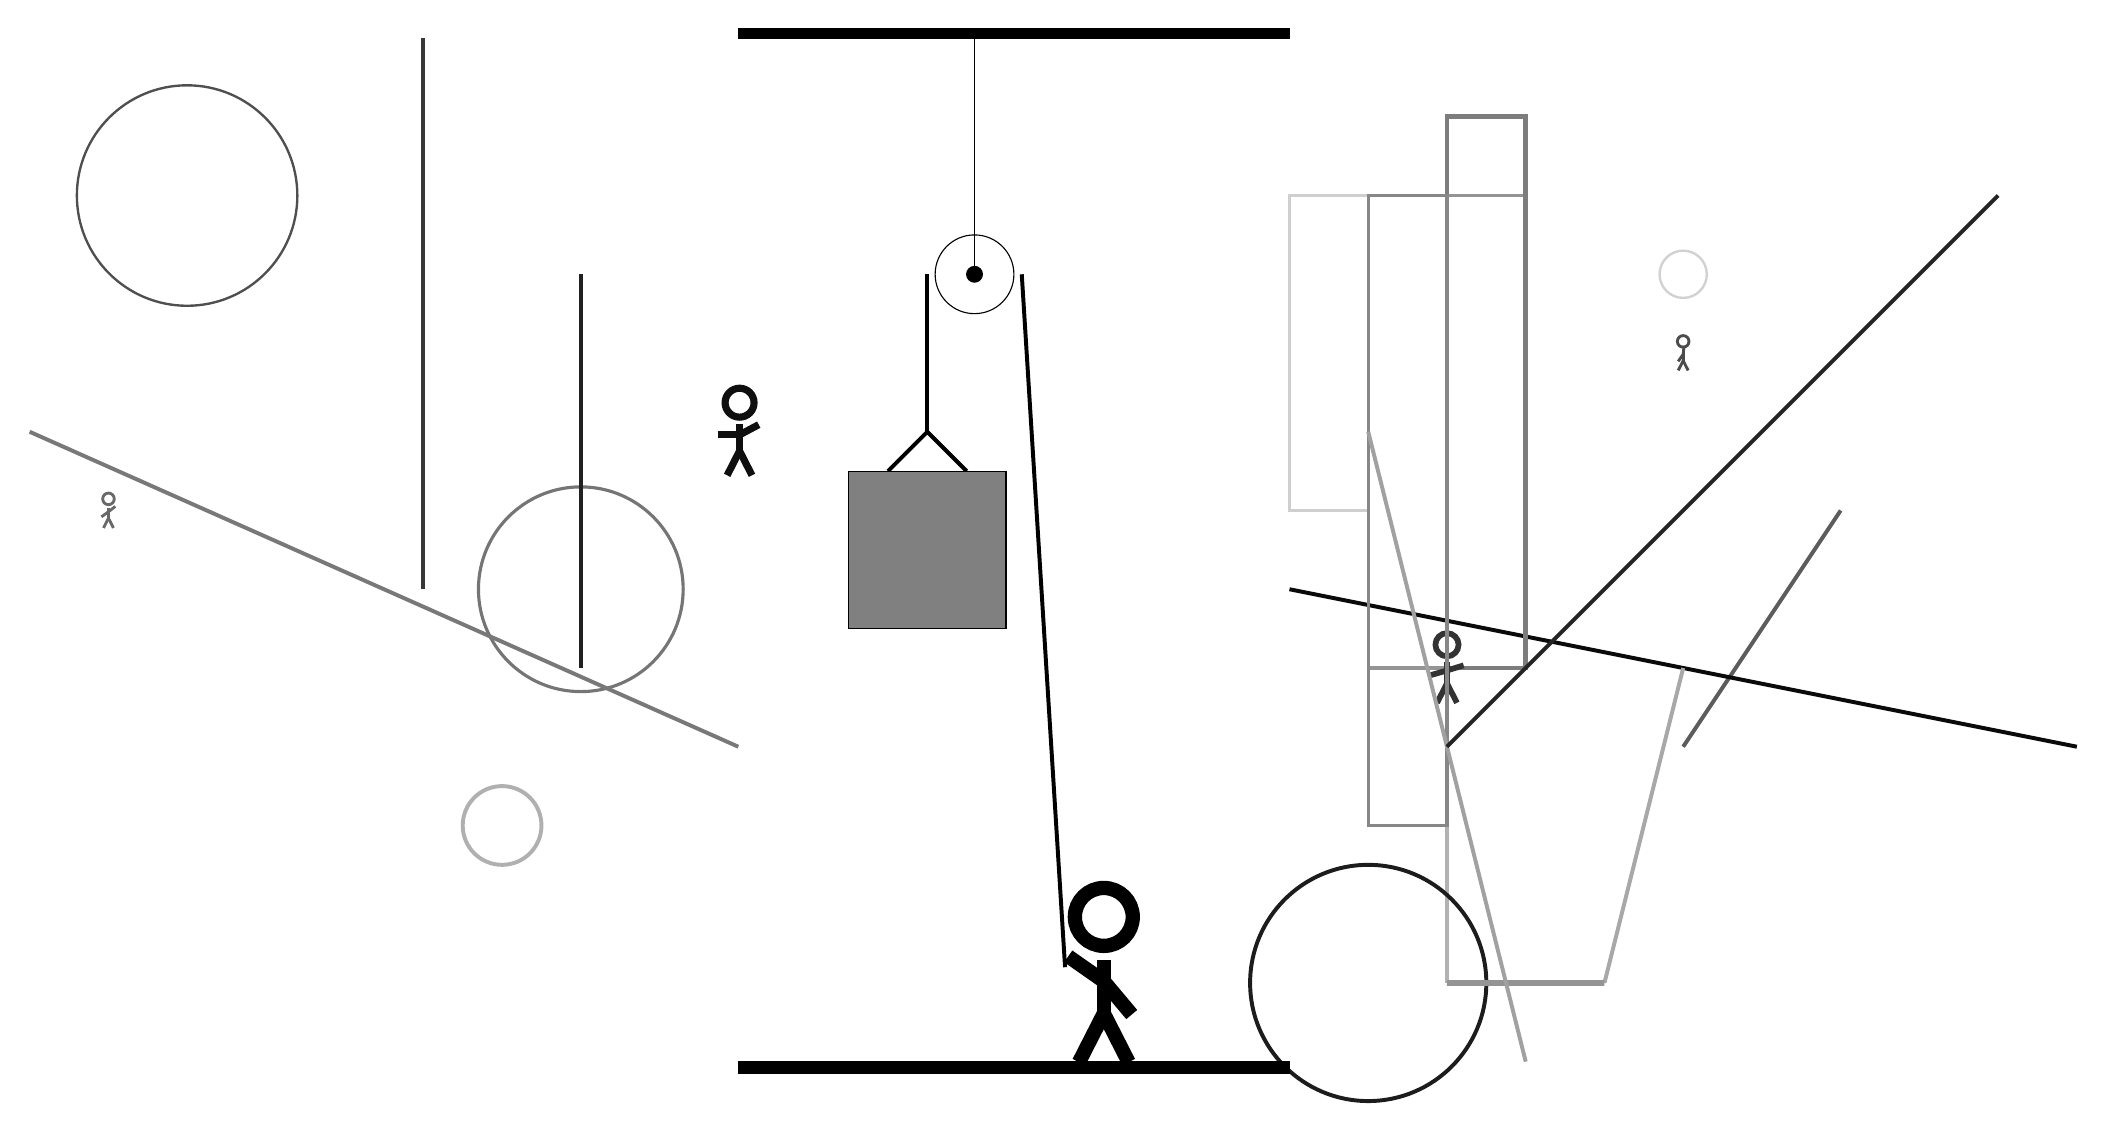
\begin{tikzpicture}
		%%%%% START %%%%%
		
		\draw[fill=black] (-2, 10) rectangle (5, 10.125);
		
		\draw[line width=0.4mm, color=black!19] (5, 4) rectangle (6, 8);
		
		\draw[line width=0.6mm, color=black!30] (7, 7) rectangle (7, -2);
		\draw[line width=0.5mm, color=black!64](10, 1) -- (12, 4);
		\draw[line width=0.5mm, color=black!96](5, 3) -- (15, 1);
		\draw[line width=0.4mm, color=black!42] (6, 8) rectangle (8, 2);
		\draw[line width=0.5mm, color=black!78](-6, 3) -- (-6, 10);
		\draw [line width=0.4mm, color=black!54](-4, 3) circle (1.3);
		\draw[line width=0.6mm, color=black!51] (7, 9) rectangle (8, 2);
		\node[line width=0.4mm, color=black!80] at (7, 2) {\Strichmaxerl[4][16][17]};
		\draw[line width=0.5mm, color=black!34](9, -2) -- (10, 2);
		
		\draw[line width=0.5mm, color=black!87](-4, 7) -- (-4, 2);
		\draw [line width=0.3mm, color=black!69](-9, 8) circle (1.4);
		\draw [line width=0.3mm, color=black!18](10, 7) circle (0.3);
		\draw [line width=0.5mm, color=black!89](6, -2) circle (1.5);
		\draw[line width=0.7mm, color=black!42] (7, -2) rectangle (9, -2);
		\node[line width=0.7mm, color=black!94] at (-2, 5) {\Strichmaxerl[5][0][28]};
		
		\draw[line width=0.4mm, color=black!47] (6, 8) rectangle (7, 0);
		
		\draw[line width=0.5mm, color=black!53](-2, 1) -- (-11, 5);
		\node[line width=0.4mm, color=black!59] at (-10, 4) {\Strichmaxerl[2][36][38]};
		
		\draw[line width=0.5mm, color=black!37](6, 5) -- (8, -3);
		\draw[line width=0.5mm, color=black!86](7, 1) -- (14, 8);
		
		\node[line width=0.3mm, color=black!70] at (10, 6) {\Strichmaxerl[2][55][84]};
		\draw [line width=0.5mm, color=black!31](-5, 0) circle (0.5);
		
		\draw (1, 7) circle (0.5);
		\draw[fill=black] (1, 7) circle (0.1);
		\draw (1, 10) -- (1, 7);
		
		\draw[line width=0.5mm] (-0.1, 4.5) -- (0.4, 5.0) -- (0.9, 4.5);
		\draw[fill=black!50] (-0.6, 4.5) rectangle (1.4, 2.5);
		
		\draw[line width=0.5mm] (0.4, 7) -- (0.4, 5.0);
		\centerarc[line width=0.5mm](1, 7)(0:180:0.6);
		\draw[line width=0.5mm](1.6, 7) -- (2.15, -1.8);
		
		\node at (2.6, -1.9) {\Strichmaxerl[10][-35][-50]};
		
		\draw[fill=black] (-2, -3) rectangle (5, -3.15);
		
		%%%%% END %%%%%
	\end{tikzpicture}
\end{document}